\subsection{Problem 3 - Inequality Constrained Quadratic Programming}
From page 475 in Nocedal and Wright the following system is given.
\begin{equation}
\begin{split}
\min_{x} q(x) = (x_1-1)^2+(x_2-2.5)^2 \\
s.t. x_1-2x_2+2> = 0,\\
-x_1-2x_2+6>=0,\\
-x_1+2x_2+2>=0,\\
x_1>=0,\\
x_2>=0.
\end{split}
\end{equation}
in MatLab a contour plot of this is made and seen in figure~\ref{fig:exe3_contour_plot}.
\begin{figure}[H]
	\centering
		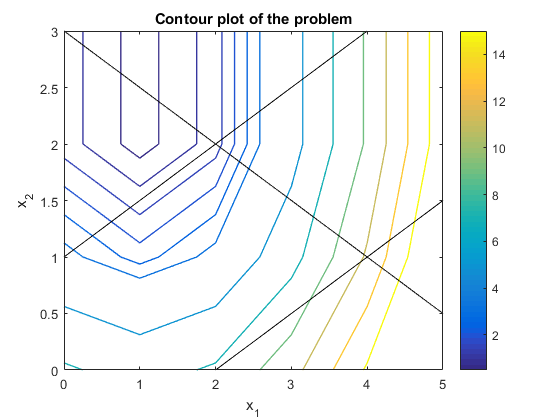
\includegraphics{exe3_contour_plot.png}
	\caption{A contour plot of the problem.}
	\label{fig:exe3_contour_plot}
\end{figure}
From the line it is seen that the feasible region is a pentagon.\\
The problem can be written in the standart martix way as:
\[H=\begin{bmatrix}
	2 & 0 \\0 & 2
\end{bmatrix}\]
\[g=\begin{bmatrix}
	-2 \\-5
\end{bmatrix}\]
\[A=\begin{bmatrix}
	1 & -1 & -1 & 1 & 0 \\
	-2 & -2 & 2 & 0 & 1
\end{bmatrix}\]
\[b= \begin{bmatrix}
	-2 \\-6 \\-2 \\0 \\0 \\
\end{bmatrix}\]
Then the general KKT system can be written as:
\[\begin{bmatrix}
	H & -A \\A^T & 0
\end{bmatrix}\times
	\begin{bmatrix}
		x\\ \lambda
	\end{bmatrix}=
		\begin{bmatrix}
			-g\\ b
	\end{bmatrix}\]
When the system can be solve with the same QP solver as used for problem 1. That gives:
\[x=\begin{bmatrix}
	-2 \\ 0
\end{bmatrix}\]

\[\lambda=\begin{bmatrix}
	0 \\1.8 \\-0.3 \\-2.1 \\ 3.0
\end{bmatrix}\]
Where all the values are multiply with 10 in the power of 16. 
\\A way to found the optimal solution is with an active set algorithm. This is applyed as the one in the Example 16.4 in N and W. The algorithm is seen in the MatLab code and the contour plot with the four different workingset are seen in figure \ref{fig:exe3_contour_plot_workingset} below. 
\begin{figure}[H]
	\centering
		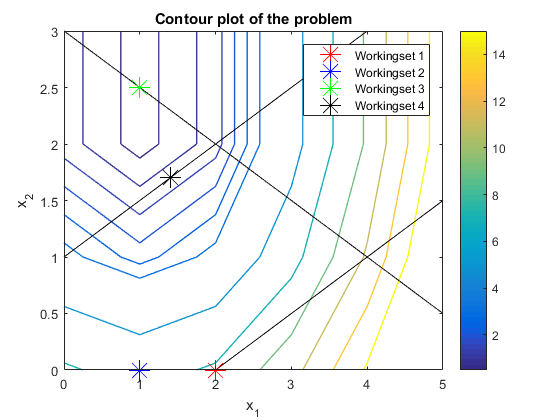
\includegraphics[scale=0.65]{exe3_contour_plot_workingset.png} 
	\caption{A contour plot of the problem, with the working set applyed .}
	\label{fig:exe3_contour_plot_workingset}
\end{figure} 
